\documentclass[aps,unsortedaddress]{revtex4-1}
\usepackage{graphicx}
\usepackage{dcolumn}
\usepackage{bm}
%\usepackage{subfig}
\usepackage[utf8]{inputenc}
\usepackage{amssymb}
\usepackage{placeins}
\usepackage{amsmath}
\usepackage{amsthm}
\usepackage{commath}
\usepackage{subcaption}
\usepackage[margin=1in]{geometry}
\usepackage[citecolor=blue,colorlinks=true,linkcolor=blue]{hyperref}

\newcommand{\partder}[2]{\dfrac{\partial  #1}{\partial  #2}} 
\newcommand{\der}[2]{\dfrac{d #1}{d  #2}}

\begin{document}

\title{Adjoint methods for gradient-based coil-winding surface optimization}
\author{E. J. Paul}
\affiliation{Department of Physics, University of Maryland, College Park, MD 20742, USA}
\email{ejpaul@umd.edu}

\author{(Coauthors)}

\iffalse
\author{M. Landreman}
\affiliation{Institute for Research in Electronics and Applied Physics, University of Maryland, College Park, MD 20742, USA}

\author{A. Bader}
\affiliation{Department of Engineering Physics, University of Wisconsin, Madison, WI 53706, USA}

\author{W. Dorland}
\affiliation{Department of Physics, University of Maryland, College Park, MD 20742, USA}
\fi

\begin{abstract}
We present a method for nonlinear gradient-based optimization of the stellarator coil-winding surface. We apply the adjoint method for sensitivity derivatives of the objective function, allowing for efficient computation of gradients while eliminating the numerical noise of derivative-free algorithms. The REGCOIL (Landreman 2017 \textit{Nucl. Fusion} \textbf{57} 046003) approach is used to obtain the coil shapes on the winding surface using a current potential method. Although this approach does not directly optimize coil shapes, we are able to improve engineering properties of the coils by targeting the root-mean-squared current density in the objective function. We obtain results for the W7-X and HSX winding surfaces which simultaneously decrease the normal magnetic field on the plasma surface,  increase the volume contained by the winding surface, and improve coil metrics in comparison with the actual winding surfaces. A technique for visualization of sensitivity derivatives obtained with the adjoint method is presented, with potential applications for understanding engineering tolerances. 
\end{abstract}

\maketitle

\section{Introduction}

Stellarators confine particles by generating rotational transform produced by external coils. Their 3-dimensional nature presents great opportunity, allowing a large space within which to find optimal plasma configurations. However, producing the necessary non-axisymmetric magnetic field also presents a significant challenge to the stellarator program. Typically the magnetic field is produced by modular, nonplanar coils. The design of simple coils which can be reasonably engineered and produce a plasma with optimal physics properties is required in order for the steady-state, disruption-free confinement of optimized stellarators to be realized. 

The stellarator coil design process often assumes the presence of a target outer plasma boundary, a configuration that is optimized for magnetohydrodynamic (MHD) stability, neoclassical confinement, and profiles of rotational transform and pressure \cite{Nuhrenberg1988}. The coil shapes are then optimized such that one of the vacuum field magnetic surfaces approximately matches the desired plasma surface. In general the desired plasma configuration can not be yielded exactly due to a balance between engineering limitations and physics requirements.

% Discussion of engineering constraints
In addition to minimization of the magnetic field error, there are several factors that should be considered in the design of coils shapes. The winding surface upon which the currents lie should be sufficiently separated from the plasma surface to allow for neutron shielding to protect the coils, a blanket, vacuum vessel, and a divertor system. In a reactor, the value of the coil-plasma distance is closely tied to the tritium breeding ratio and overall cost of electricity and was targeted in the ARIES-CS study to reduce machine size \cite{Guebaly2008}. In practice the minimum feasible coil-plasma separation is a function of the desired plasma shape. In particular, concave regions (such as the bean W7-X cross section) are difficult to produce \cite{Landreman2016} and require the winding surface to be near to the plasma surface. While decreasing the inter-coil spacing minimizes ripple fields, increasing coil-coil spacing allows adequate space for maintenance, heat transport plumbing, diagnostics, and support structures. In turn, a flexible maintenance scheme ultimately determines the fraction of operational time of a reactor \cite{Waganer2008}. The curvature of a coil should be below a certain threshold to allow for the finite thickness of the conducting material and to avoid prohibitively high manufacturing costs. The length of each coil should also be considered, as its increase will also drive up manufacturing costs. Identifying coils with suitable engineering properties can impact the possible size and cost of a stellarator experiment. 

The first tool for stellarator coil design assumed the coils to lie on a closed toroidal winding surface enclosing the desired plasma surface. In \texttt{NESCOIL} \cite{Merkel1987}, the surface currents on this surface are determined by minimizing the integral-squared normal magnetic field on the target plasma surface. Using a stream function approach, the current potential on the winding surface is decomposed in Fourier harmonics. This takes the form of a least-squares problem which can be solved with a single linear system. The coil filament shapes can be obtained from the contours of the current potential. Because it is guaranteed to find a local minimum, \texttt{NESCOIL} is often used in the prelimiary stages of the design process \cite{Spong2010, Ku2011, Drevlak2013} and was used for initial coil configuration studies for W7-X \cite{Nuhrenberg1993} and NCSX \cite{Pomphrey2001}. However, the inversion of the Biot-Savart integral by \texttt{NESCOIL} is fundamentally ill-posed, resulting in solutions with amplified noise. The \texttt{REGCOIL} \cite{Landreman2017} approach addresses this problem with Tikhonov regularization. Here the surface-average-squared current density, corresponding to the inverse distance between coils, is added to the objective function. With the addition of this regularization term, \texttt{REGCOIL} is able to simultaneously increase the minimum coil-coil distances and improve reconstruction of the desired plasma surface over \texttt{NESCOIL} solutions. 

In this work we build on the \texttt{REGCOIL} method to optimize the current distribution in 3 dimensions. The current distribution on a single winding surface is computed with \texttt{REGCOIL}, and the winding surface geometry is optimized to reproduce the plasma surface with fidelity and improve engineering properties of the coil shapes. The complexity of the nonlinear optimization is reduced over other approaches, as the current distribution on the winding surface is efficiently and robustly computed by solving a linear system.  

Other nonlinear coil optimization tools exist which evolve discrete coil shapes rather than continuous surface current distributions. Drevlak's \texttt{ONSET} code \cite{Drevlak1998} extended upon the \texttt{NESCOIL} code to optimize coil shapes within limiting inner and outer coil surfaces. The \texttt{COILOPT} \cite{Strickler2002,Strickler2004} code optimizes coil filaments on a winding surface and was developed for the design of the NCSX coilset \cite{Zarnstorff2001}. \texttt{COILOPT++} \cite{Brown2015} improved upon \texttt{COILOPT}, allowing one to straighten module coils to ease access to plasma components. The need for a winding surface was eliminated with the \texttt{FOCUS} \cite{Zhu2017} code, which represents coils as three-dimensional space curves. The \texttt{FOCUS} approach employs analytic differentiation for gradient-based optimization, as we do in this work. 

% ref. 10-14 in Matt's paper (applications of NESCOIL)
% W7X - Nuhrenberg (don't think NESCOIL was used

% In the design of the W7-X coil set, \texttt{NESCOIL} was used to obtain contours of the current potential on the coil-winding surface, which were then smoothed to form coil filament shapes

Many engineering design problems can be formulated in terms of the minimization of an objective function with respect to some free parameters. A powerful tool for such problems is gradient-based optimization, which requires knowledge of the sensitivity of the objective function with respect to design parameters. If the optimization space is very large, finite differencing of an objective function with respect to all of the free parameters to obtain the gradients can be expensive and introduces additional noise. Although derivative-free optimization techniques exist, they are limited in the types of constraints that can be implemented and are typically effective only for small problems \cite{Nocedal2006}. Adjoint methods allow for efficient computation of gradients of the objective function with respect to a large number of design parameters. The cost of computing the sensitivity derivatives in this way scales independently of the number of design parameters and linearly with the number of objective functions. In addition to gradient-based optimization, these sensitivity derivatives can also be used for uncertainty quantification in scientific computation \cite{Roy2011} or to construct sensitivity maps for visualization of how an objective function changes with respect to normal displacements of a surface \cite{Othmer2008,Othmer2014}. 

Adjoint methods were developed in the 1970s for sensitivity analysis of drag and flow dynamics \cite{Pironneau1974} and have been widely used for shape optimization in the field of aerodynamics and computation fluid dynamics (CFD) \cite{Kuruvila1995,Jameson1998,Anderson1999,Othmer2008,Othmer2014}. Only recently have these methods been utilized for tokamak physics in the context of advanced divertor design with plasma edge simulations \cite{Baelmans2017} and for fitting model parameters with experimental edge data on ASDEX-Upgrade \cite{Kim2001}. As stellarator design introduces many additional geometric parameters over tokamak design, adjoint-based optimization could provide a significant reduction in computational cost to this field. 

%They have also been applied to determine model parameters from geophysical data \cite{Plessix2006}. 

The design of magnetic resonance imaging (MRI) coils has also benefited from adjoint methods \cite{Jia2014}. 
Gradient coils which lie on a winding surface must provide a specified spatial variation in the magnetic field within a region of interest. This inverse problem is often solved with a linear least-squares system by minimizing the squared departure from the desired field at specified points with respect to the current in differential surface elements \cite{Turner1993}. This is analogous to the \texttt{NESCOIL} \cite{Merkel1987} approach. This approach was improved by the addition of a regularization term related to the integrated-squared current density \cite{Forbes2005} or the integral-squared curvature \cite{Forbes2001}, analogous to the \texttt{REGCOIL} approach. The adjoint approach is applied to compute the sensitivity of an objective function with respect to the current potential on the winding surface. Here the Biot-Savart law is written in terms of a matrix inversion using the least-squares finite element method, and the adjoint of this matrix is inverted to compute the sensitivity derivatives \cite{Jia2014}. As the adjoint formalism has proven fruitful in this field, we anticipate that it could have similar applications in the closely-related field of stellarator coil design. 

We present a new method for design of the coil-winding surface using adjoint-based optimization. An adjoint solve is performed to obtain gradients of several figures of merit, the integrated-squared normal magnetic field on the plasma surface and root-mean-squared current density on the winding surface, with respect to the Fourier components describing the coil surface. The optimization method and objective function are described in section \ref{sect_opt}. The adjoint method for computing gradients of the objective function is described in section \ref{sect_adjoint} and a brief overview of the \texttt{REGCOIL} approach is given in \ref{section_REGCOIL}. Optimization results for the W7-X and HSX winding surfaces are presented in section \ref{sect_results}. In \ref{sect_sensitivity} we demonstrate a method for visualization of shape derivatives on the winding surface. In section \ref{sect_conclusions} we will summarize our results and conclude. 

\section{Winding surface optimization}
\label{sect_opt}

\subsection{Objective function}
The cartesian components of the winding surface can be decomposed in Fourier harmonics.
\begin{gather}
x' = \sum_{m,n} r_{mn}^c \cos(m \theta' - n N_p \zeta') \cos (\zeta') \\
y' = \sum_{m,n} r_{mn}^c \cos(m \theta' - n N_p \zeta') \sin (\zeta') \\
z' = \sum_{m,n} z_{mn}^s \sin(m \theta' - n N_p \zeta') 
\label{Fourier}
\end{gather}
Here $N_p$ is the number of toroidal periods, $\zeta'$ is the normal toroidal angle, and $\theta'$ is a poloidal angle. We take the Fourier components of the winding surface, $\Omega = (r_{mn}^c, z_{mn}^s)$, as our optimization parameters and assume a desired plasma surface to be held fixed. Once the winding surface geometry is determined, our task is to obtain the surface current density, $\bm{K}$. The divergentless surface current density can be related to a scalar current potential, $\Phi$, the stream function for $\bm{K}$.
\begin{gather}
\bm{K} = \bm{n}' \times \nabla \Phi
\end{gather}
Here $\bm{n}'$ is the unit normal on the winding surface. For a given winding surface geometry, $\Omega$, and desired plasma surface, the current potential $\Phi (\Omega)$ can be determined by solving the \texttt{REGCOIL} system to obtain a solution which both reproduces the desired plasma surface with fidelity and maximizes coil-coil distance, as described in section \ref{section_REGCOIL}.

We define an objective function, $f$, which will be minimized with respect to $\Omega$. 
\begin{gather}
f(\Omega, \Phi(\Omega))  = \chi^2_B(\Omega, \Phi(\Omega)) - \alpha_1 V_{\text{coil}}^{1/3}(\Omega) + \alpha_2 S_p(\Omega) + \alpha_3  \norm{\bm{K}}_2(\Omega, \Phi(\Omega))
\label{objective_function}
\end{gather}
The objective function depends on $\Phi$, the current potential on the surface, and $\Omega$, the geometric properties of the coil-winding surface. The quantity $\chi^2_B$ is the surface-average-squared normal magnetic field on the desired plasma surface,
\begin{gather}
\chi^2_B = \int_{\text{plasma}} d^2 A \, B_n^2.
\label{chi2_B}
\end{gather}
The normal component of the magnetic field on the plasma surface, $B_n$, includes contributions from currents in the plasma, current density $\bm{K}$ on the winding surface, and currents due to other external coils. This depends on both the geometric properties of the surface and the current distribution on the surface. The quantity $V_{\text{coil}}$ is the total volume enclosed by the coil-winding surface.
\begin{gather}
V_{\text{coil}} = \int_{\text{coil}} d^3 V
\end{gather}
We use $V_{\text{coil}}$ as a proxy for coil-plasma separation. The quantity $S_p$ is a measure of the spectral condensation of the coil-winding surface \cite{Hirshman1985}. 
\begin{gather}
S_p = \sum_{m,n} m^{p} \left( (r_{mn}^c)^2 + (z_{mn}^s)^2 \right)
\end{gather}
Smaller values of $S_p$ correspond to Fourier spectra which decay rapidly with increasing $m$. We take advantage of the non-uniqueness of the representation in equation \ref{Fourier} to obtain surface parameterization which are represented more efficiently. While $\zeta'$ is the normal toroidal angle, for a given surface $\theta'$ can be defined many ways depending on the Fourier representation. % Will we show this?
Minimization of $S_p$ produces surfaces for which the poloidal angle approaches a constant arclength angle. We use a typical value of $p=2$. The quantity $\norm{\bm{K}}_2$ is the vector 2-norm of the current density, defined in terms of an area integral over the surface. 
\begin{gather}
\norm{\bm{K}}_2 = \left( \frac{\int_{\text{coil}} d^2 A \, \abs{\bm{K}}^2}{\int_{\text{coil}} d^2 A}  \right)^{1/2}
\end{gather}
Although we are using a current potential approach rather than directly optimizing coil shapes, including $\norm{\bm{K}}_2$ in the objective function allows us to indirectly obtain winding surfaces which allow for coils with good engineering properties. 

To demonstrate this, we compute the coilset on the actual W7-X winding surface using \texttt{REGCOIL}. The regularization parameter, $\lambda$, is chosen to achieve several values of $\norm{\bm{K}}_2$. Coil shapes are obtained from the contours of $\Phi$. In figure \ref{rmsKcoilcompare}, 2 of the W7-X non-planar coils computed in this way are shown, and the corresponding average (over the 5 coil set) metrics are shown in table \ref{rmsKcoilmetrics}. We consider the length, $l$, toroidal extent, $\Delta \zeta'$, and curvature $\kappa$. Although the metrics associated with individual coils may not necessarily improve, the mean length, toroidal extent, and curvature decrease as $\norm{\bm{K}}_2$ decreases. Here the curvature, $\kappa$, of a 3-dimensional parameterized curve, $\bm{r}(t)$, is defined in the following way.
\begin{gather}
\kappa = \frac{\bigg \rvert \der{\bm{r}}{t} \times \der{^2 \bm{r}}{t^2} \bigg \rvert}{\bigg \rvert \der{\bm{r}}{t} \bigg \rvert^3}
\end{gather}

\FloatBarrier
\begin{figure}
\begin{subfigure}[b]{0.3\textwidth}
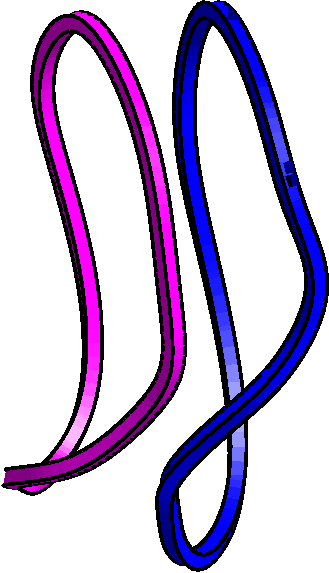
\includegraphics[width=0.57\textwidth]{target_2_2e6.pdf}
\caption{$\norm{\bm{K}}_2 = 2.2$ MA/m}
\end{subfigure}
\begin{subfigure}[b]{0.3\textwidth}
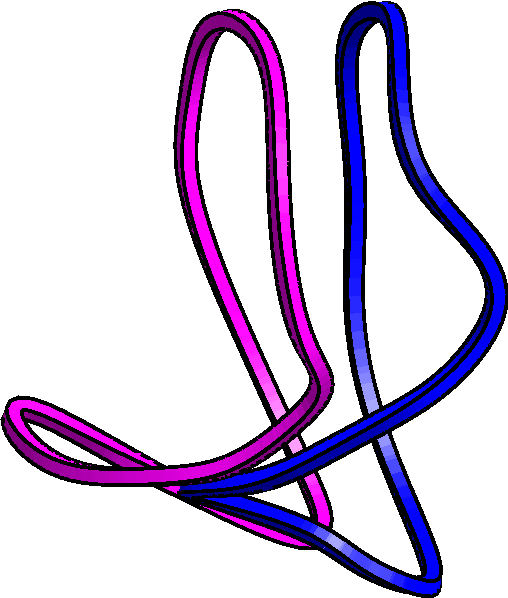
\includegraphics[width=0.84\textwidth]{target_2_7e6.pdf}
\caption{$\norm{\bm{K}}_2 = 2.7$ MA/m}
\end{subfigure}
\begin{subfigure}[b]{0.3\textwidth}
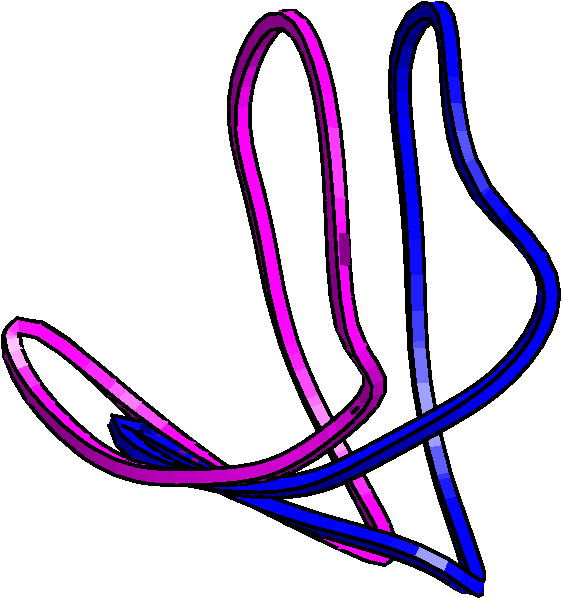
\includegraphics[width=0.95\textwidth]{target_3_2e6.pdf}
\caption{$\norm{\bm{K}}_2 = 3.2$ MA/m}
\end{subfigure}
\caption{Two non-planar W7-X coils computed with \texttt{REGCOIL} using the actual W7-X winding surface. The regularization parameter $\lambda$ is chosen to achieve the shown values of $\norm{\bm{K}}_2$. As $\norm{\bm{K}}_2$ increases, the mean length, toroidal extent, and curvature decrease.}
\label{rmsKcoilcompare}
\end{figure}

\begin{table}
\renewcommand{\arraystretch}{1.4}
\begin{tabular} { | c | c | c | c | }
\hline
$\norm{\bm{K}}_2$ [MA/m] & Mean $l$ [m] & Mean $\Delta \zeta'$ [rad.] & Mean $\kappa$ [m$^{-1}$] \\ \hline 
2.2 & 8.028 & 0.146 & 0.954 \\ \hline
2.7 & 9.168 & 0.222 & 1.138 \\ \hline
3.2 & 11.518 & 0.305 & 1.265 \\ \hline
\end{tabular}
\caption{Comparison of metrics for coils computed with \texttt{REGCOIL} using the actual W7-X winding surface. The regularization parameter $\lambda$ is varied to achieve these values of $\norm{\bm{K}}_2$.}
\label{rmsKcoilmetrics}
\end{table}
\FloatBarrier

The relative weights in equation \ref{objective_function} ($\alpha_1$, $\alpha_2$, and $\alpha_3$) are chosen such that each of the terms in the objective function have roughly similar magnitudes, though much tuning of these parameters is required to obtain results which simultaneously improve the physics properties (decrease $\chi^2_B$) and engineering properties (increase $V_{\text{coil}}$, decrease $\kappa$ and $\Delta \zeta'$).

\subsection{Optimization constraints}
\label{sect_constraint}

Minimization of $f$ is performed subject to the inequality constraint $d_{\text{min}} \geq d_{\text{min}}^{\text{target}}$. Here $d_{\text{min}}$ is the minimum distance between the coil-winding surface and the plasma surface,
\begin{gather}
d_{\text{min}} = \min_{\theta',\zeta'} \left( d_{\text{coil-plasma}} \right) = \min_{\theta',\zeta'} \left( \min_{\theta, \zeta} \left( \norm{ \bm{r} - \bm{r}' } \right) \right),
\end{gather}
and $d_{\text{min}}^{\text{target}}$ is the minimum tolerable coil-plasma separation. Here $\theta$ and $\zeta$ are poloidal and toroidal angles on the plasma surface, $\bm{r}$ and $\bm{r}'$ are the position vectors on the plasma and winding surface respectively, and $d_{\text{coil-plasma}}$ is the coil-plasma distance as a function of $\theta'$ and $\zeta'$. 

The maximum current density, $K_{\text{max}}$, is also constrained. 
\begin{gather}
K_{\text{max}} = \max_{\theta',\zeta'} \left( \abs{\bm{K}} \right)
\end{gather}
This corresponds to a fixed minimum coil-coil spacing. This constraint is enforced by fixing $K_{\text{max}}$ to obtain the regularization parameter $\lambda$ in the \texttt{REGCOIL} solve, so we avoid the need for an equality constraint or the inclusion of $K_{\text{max}}$ in the objective function. Rather, $\Phi(\Omega)$ is determined such that $K_{\text{max}}$ is fixed. The inequality-constrained nonlinear optimization is performed using the NLOPT \cite{NLOPT} software package using a conservative convex separable approximation \cite{Svanberg2002}. 

\section{Overview of the REGCOIL system}
\label{section_REGCOIL}

The current potential $\Phi$ can be decomposed into single-valued and secular terms.
\begin{gather}
\Phi(\theta', \zeta') = \Phi_{\text{sv}}(\theta',\zeta') + \frac{ G \zeta'}{2 \pi} + \frac{I \theta'}{2 \pi}
\end{gather}
The secular terms are determined from the currents linking the coil surface poloidally and toroidally, while the single-valued term ($\Phi_{\text{sv}}$) is determined by solving the \texttt{REGCOIL} system. The single-valued current potential is chosen to minimize the primary objective function, $\chi^2$.
\begin{gather}
\chi^2 = \chi^2_B - \lambda \chi^2_K
\label{primary_objective}
\end{gather}
Here $\chi^2_K$ is the surface-average-squared current density on the winding surface,
\begin{gather}
\chi^2_K = \int_{\text{coil}} d^2A \, \abs{\bm{K}}^2,
\end{gather}
and $\chi^2_B$ is defined in equation \ref{chi2_B}. The regularization parameter $\lambda$ is chosen to obtain the target $K_{\text{max}}$. This problem is discretized by expanding $\Phi_{\text{sv}}$ in a finite Fourier series.
\begin{gather}
\Phi_{\text{sv}}(\theta',\zeta') = \sum_j \Phi_j \left( \begin{array}{c} \sin \\ \cos \end{array} \right)_j (m_j \theta' - n_j \zeta')
\end{gather}
For a stellarator symmetric configuration, only the sine series is needed. As the minimization of $\chi^2$ with respect to $\Phi_{j}$ is a convex linear least-squares problem, it can be solved via the normal equations to obtain a unique solution. The Fourier amplitudes, $\Phi_j$, are determined by solving a linear system,
\begin{gather}
\sum_k A_{j,k} \Phi_k = b_j,
\label{forward}
\end{gather}
such that $\chi^2$ is minimized,
\begin{gather}
\partder{\chi^2}{\Phi_k} = \partder{\chi^2_B}{\Phi_k} + \lambda \partder{\chi^2_K}{\Phi_k} = 0.
\label{regcoil_minimization}
\end{gather}
For additional details see \cite{Landreman2017}.

\section{Sensitivity Derivatives and Adjoint Formalism}
\label{sect_adjoint}
We must compute sensitivity derivatives of $f$ with respect to the geometric components, $\Omega$, in order to use gradient-based optimization methods. The spectral condensation function, $S_p$, and volume, $V_{\text{coil}}$, are explicit functions of $\Omega$, so their analytic derivatives can be obtained. On the other hand, $\chi^2_B$ and $\norm{\bm{K}}_2$ depend both explicitly on coil geometry and on $\Phi(\Omega)$. One approach to obtain the sensitivity derivatives of these quantities could be to solve the \texttt{REGCOIL} linear system $N_{\Omega} +1$ times, taking a finite difference step in each Fourier coefficient. However, if $N_{\Omega}$ (number of Fourier modes) is large, the computational cost of this method could be prohibitively expensive. Instead we will apply the adjoint method to compute sensitivity derivatives. This technique will be demonstrated below. 

The sensitivity derivative of $\chi^2_B$ can be computed using the chain rule. 
\begin{gather}
\partder{\chi^2_B(\Omega, \bm{\Phi}(\Omega))}{\Omega_j} \bigg \rvert_{A \bm{\Phi} = \bm{b}} = \partder{\chi^2_B}{\Omega_j} \bigg \rvert_{\bm{\Phi}} + \partder{\chi^2_B}{\bm{\Phi}} \cdot \partder{\bm{\Phi}}{\Omega_j} \bigg \rvert_{A \bm{\Phi} = \bm{b}}
\label{sensitivity_der}
\end{gather}
The dot product is a contraction over the current potential basis functions, $\Phi_k$. We can compute $\partial \bm{\Phi}/ \partial \Omega_j$ by differentiating the linear system, equation \ref{forward}, with respect to $\Omega_j$ and inverting the operator, $A$.
\begin{gather}
\partder{A}{\Omega_j} \bm{\Phi} + A \partder{\bm{\Phi}}{\Omega_j} = \partder{\bm{b}}{\Omega_j} \\
\partder{\bm{\Phi}}{\Omega_j} = A^{-1} \left( \partder{\bm{b}}{\Omega_j} - \partder{A}{\Omega_j} \bm{\Phi} \right) 
\label{linear_sensitivity}
\end{gather}
Equation \ref{linear_sensitivity} is inserted into equation \ref{sensitivity_der}.
\begin{gather}
\partder{\chi^2_B(\Omega, \bm{\Phi}(\Omega))}{\Omega_j} \bigg \rvert_{A \bm{\Phi} = \bm{b}} = \partder{\chi^2_B}{\Omega_j} \bigg \rvert_{\bm{\Phi}} + \partder{\chi^2_B}{\bm{\Phi}} \cdot \left[ A^{-1} \left( \partder{\bm{b}}{\Omega_j} - \partder{A}{\Omega_j} \bm{\Phi} \right) \right] 
\end{gather}
The sensitivity derivatives could be obtained by inverting $A$ for each of the geometric components $\Omega_j$ and performing the inner product with $\partial \chi^2_B/ \partial \bm{\Phi}$ for each $\Omega_j$. However, the computational cost of this method scales similarly to that of finite differencing. Instead, we can exploit the adjoint property of the operator. For a given inner product, the adjoint of an operator, $A$, is defined such that $(b,Ac) = (A^{\dagger} b, c)$. As we are working in $\mathbb{R}^n$, the adjoint operator corresponds to the matrix transpose. 
\begin{gather}
\partder{\chi^2_B(\Omega, \bm{\Phi}(\Omega))}{\Omega_j} \bigg \rvert_{A \bm{\Phi} = \bm{b}} = \partder{\chi^2_B}{\Omega_j} \bigg \rvert_{\bm{\Phi}} + \left[ \left(A^{-1}\right)^{T} \partder{\chi^2_B}{\bm{\Phi}}\right] \cdot \left( \partder{\bm{b}}{\Omega_j} - \partder{A}{\Omega_j} \bm{\Phi} \right)
\end{gather}
For any invertible matrix, $\left( A^{-1} \right)^T = \left( A^{T} \right)^{-1}$. So, we can instead invert the operator $A^T$ to compute an adjoint variable, $\bm{q}$.
\begin{gather}
A^T \bm{q} = \partder{\chi^2_B}{\bm{\Phi}}
\label{adjoint}
\end{gather}
Rather than finite difference in each $\Omega_j$ or invert $A$ for each $\partial \bm{\Phi}/\partial \Omega_j$ as in equation \ref{linear_sensitivity}, we simply solve two linear systems: the forward (equation \ref{forward}) and adjoint (equation \ref{adjoint}). The adjoint equation is similar to the forward equation ($A^T$ has same dimensions and eigenspectrum), so the same computational tools can be used to solve the adjoint problem. We perform an inner product with $\bm{q}$ to obtain the sensitivity derivatives with respect to each $\Omega_j$. 
\begin{gather}
\partder{\chi^2_B(\Omega, \bm{\Phi}(\Omega))}{\Omega_j} \bigg \rvert_{A \bm{\Phi} = \bm{b}} = \partder{\chi^2_B}{\Omega_j} \bigg \rvert_{\bm{\Phi}} + \bm{q} \cdot \left( \partder{\bm{b}}{\Omega_j} - \partder{A}{\Omega_j} \bm{\Phi} \right)
\label{adjointsensitivity}
\end{gather}
The derivatives $\partial \bm{b}/\partial \Omega_j$, $\partial A/\partial \Omega_j$, $\left( \partial \chi^2_B/\partial \Omega_j \right)_{\bm{\Phi}}$, and $\partial \chi^2_B/\partial \bm{\Phi}$ can be computed analytically. In the above discussion, the regularization parameter $\lambda$ has been assumed to be fixed. A similar method can be used if a $\lambda$ search is performed to obtain a target $K_{\text{max}}$ (see appendix \ref{lambda_search}). The same method is used to compute sensitivity derivatives of $\norm{\bm{K}}_2$. 

\iffalse
The gradients of $\chi^2_B$ at fixed $K_{\text{max}}$ have been benchmarked against finite differencing.
\FloatBarrier
\begin{figure}
\includegraphics[width=.8\textwidth]{finite_differencing.pdf}
\caption{The gradient of $\chi^2_B$ with respect to the Fourier components of the winding surface, $\Omega$, computed with \texttt{REGCOIL} using the adjoint method are compared with finite differencing.}
\end{figure}
\FloatBarrier
\fi

The constraint functions, $d_{\text{min}}$ and $K_{\text{max}}$, must also be differentiated with respect to $\Omega_j$. As $d_{\text{min}}$ is defined in terms of the minimum function, we approximate it using the smooth log-sum-exponent function \cite{Boyd2004}.
\begin{gather}
d_{\text{min, lse}} = - \frac{1}{p} \log \left( \sum_{i_{\theta}}^{N_{\theta}} \sum_{i_{\zeta}}^{N_{\zeta}} \sum_{i_{\theta'}}^{N_{\theta'}} \sum_{i_{\zeta'}}^{N_{\zeta'}} \, \exp \left( - p \sqrt{(\bm{r}' - \bm{r})^2} \right) \right)
\label{lse_d}
\end{gather}
As $p$ approaches infinity, $d_{\text{min, lse}}$ approaches $d_{\text{min}}$. For $p$ very large, the function obtains very sharp gradients. A typical value of $p = 10^4$ was used. This function can be analytically differentiated with respect to $\Omega_j$. The log-sum-exponent function is also used to approximate $K_{\text{max}}$. 

\section{Winding surface optimization results}
\label{sect_results}

\subsection{Trends with optimization parameters}
\FloatBarrier

Beginning with the actual W7-X winding surface, we perform scans over the coefficients ($\alpha_1$ and $\alpha_2$) in the objective function, equation \ref{objective_function}. The constraint tolerance, $d_{\text{min}}^{\text{target}}$, is set to be the distance of closest approach on the initial winding surface. The cross sections of the optimized surfaces in the poloidal plane are shown in figures \ref{alpha1_scan} and \ref{alpha2_scan} along with the last-closed flux surface (red), initial winding surface (black solid), and a constant offset surface at $d_{\text{min}}^{\text{target}}$ (black dashed). As $\alpha_1$ increases with fixed $\alpha_2 = 0.3$ and $\alpha_3 = 0$, $d_{\text{coil-plasma}}$ increases significantly on the outboard side while it remains fixed at the inboard concave regions. The winding surface obtains a somewhat pointed shape at the triangle cross-section ($\zeta' = 0.5$ $2\pi/N_p$), a region where the plasma surface has sharp spatial scales. At small values of $\alpha_1$ the winding surface approaches the constant offset surface. We anticipate these trends, as the shaping components of the magnetic field produced by coils decrease exponentially away from the winding surface, and only long-wavelength structures on the plasma surface are consistent with solutions to Laplace's equation which decay slowly away from the coil surface \cite{Boozer2000}. Therefore, if $\chi^2_B$ is dominant in the objective function, the coil surface will approach the plasma surface until the $d_{\text{min}}$ constraint is met. Even if $\chi^2_B$ is not the dominant term, the winding surface approaches the plasma surface in regions of small spatial scales. This effect is especially pronounced for plasma shapes with concave regions, which require a small coil-plasma separation, as characterized by the feasibility sequence \cite{Landreman2016}. With increasing $\alpha_2$ at fixed $\alpha_1 = \alpha_3 = 0$, the winding surface approaches a cylindrical torus which has a minimal Fourier spectra. At small values of $\alpha_2$ ($\chi^2_B$ dominant in objective function) the surface again approaches a constant offset surface. 

\begin{figure}
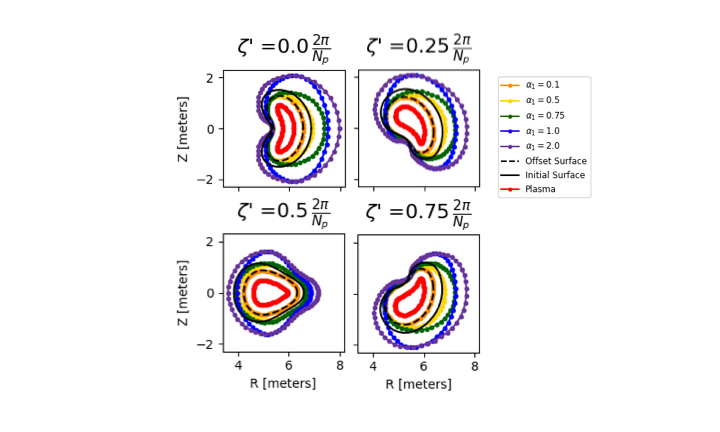
\includegraphics[width=.8\textwidth]{alpha1_scan.png}
\caption{Optimized winding surfaces obtained with $\alpha_2 = 0.3$ and $\alpha_3 = 0$. The actual W7-X winding surface is used as the initial surface in the optimization. As $\alpha_1$ increases, the magnitude of the $V_{\text{coil}}$ term in the objective function increases, and $d_{\text{coil-plasma}}$ increases on the outboard side. }
\label{alpha1_scan}
\end{figure}

\begin{figure}
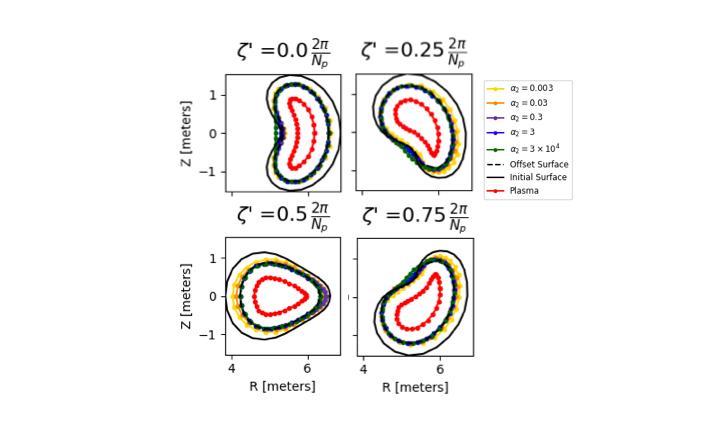
\includegraphics[width=.8\textwidth]{alpha2_scan.png}
\caption{Optimized winding surfaces obtained with $\alpha_1 = 0$ and $\alpha_3 = 0$. The actual W7-X winding surface is used as the initial surface in the optimization. As $\alpha_2$ increases, the magnitude of the spectral-width term in the objective function increases, and the winding surface approaches a cylindrical torus with a minimal Fourier spectra.}
\label{alpha2_scan}
\end{figure}

\FloatBarrier
\subsection{Optimal W7-X winding surface}
\FloatBarrier
We perform optimization as described in sections \ref{sect_opt}, beginning with the actual W7-X winding surface. The $K_{\text{max}}$ constraint is selected such that the metrics ($l$, $\kappa$, and $\Delta \zeta'$) of the coils computed on the initial surface roughly match those of the actual non-planar coilset. The constraint tolerance $d_{\text{min}}^{\text{target}}$ is set to be the minimum $d_{\text{coil-plasma}}$ on the initial winding surface. Parameters $\alpha_1 = 0.5$, $\alpha_2 = 0.24$, and $\alpha_3 = 1.6\times10^{-6}$ were used in the objective function. The optimal surface and coilset are shown in figure \ref{fig_w7x}, and the corresponding metrics are shown in table \ref{table_w7x}. We find a solution which increases $V_{\text{coil}}$ by 22\% and decreases $\chi^2_B$ by 52\% over the initial winding surface. Note that $\chi^2_B$ is nonzero on the initial winding surface as \texttt{REGCOIL} does not exactly reproduce the W7-X coilset. In addition, the optimized coilset features a smaller toroidal extent and mean curvature while fixing $K_{\text{max}}$ (coil-coil separation). The length of the coils increases to accommodate for the increase in $V_{\text{coil}}$. Again we find that the increase in $V_{\text{coil}}$ is most pronounced in the outboard convex regions. 

\FloatBarrier
\begin{figure}
\begin{subfigure}[b]{0.8\textwidth}
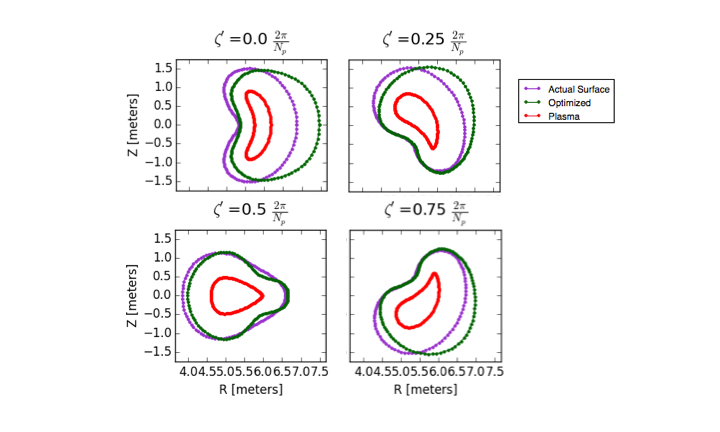
\includegraphics[width=1\textwidth]{w7x_opt_surf.png}
\caption{}
\end{subfigure}
\begin{subfigure}[b]{0.8\textwidth}
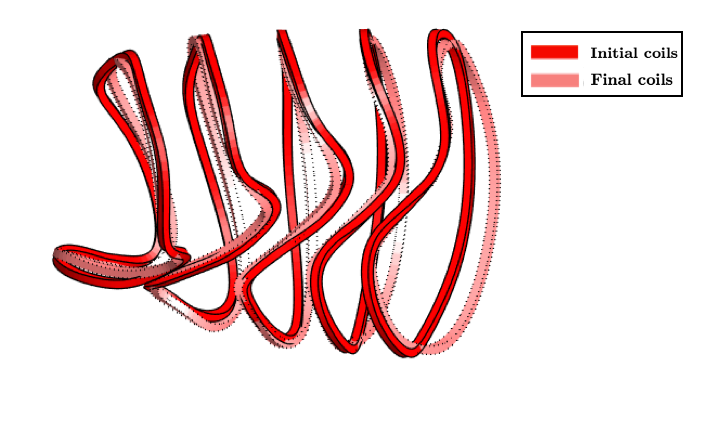
\includegraphics[width=0.8\textwidth]{w7x_opt_coils.png}
\caption{}
\end{subfigure}
\caption{(a) The actual W7-X coil-winding surface and plasma surface are shown with the optimized winding surface. In comparison with the actual surface, the optimized surface reduced $\chi^2_B$ by 52\% and increased $V_{\text{coil}}$ by 22\%. (b) Comparison of coilset computed with \texttt{REGCOIL} using the actual W7-X winding surface (dark) and the optimized surface (light).}
\label{fig_w7x}
\end{figure}

\begin{table}
\renewcommand{\arraystretch}{1.4}
\begin{tabular} {| c | c | c | c | c | c | c | c |}
\hline
& $\chi^2_B$ [T$^2$m$^2$] & $V_{\text{coil}}$[m$^3$] & $\norm{\bm{K}}_2$ [MA/m] & Mean $l$ [m] & Mean $\Delta \zeta'$ [rad.] & Mean $\kappa$ [m$^{-1}$]  \\ \hline 
Initial & 0.11 & 156.05 & 2.21 & 8.55 & 0.19 & 1.16 \\ \hline
Optimized & 0.07 & 189.76 & 2.16 & 8.75 & 0.18 & 1.04   \\ \hline
Actual coilset & & & & 8.69 & 0.20 & 1.16  \\ \hline
\end{tabular}
\caption{Comparison of metrics of winding surface and coilset for W7-X initial and optimized surfaces. The coil metrics for the actual W7-X nonplanar coils are also shown. Regularization in \texttt{REGCOIL} is chosen such that the coil metrics computed on the initial surface roughly match those of the actual coilset.}
\label{table_w7x}
\end{table}

\FloatBarrier
\subsection{Optimal HSX winding surface}
\FloatBarrier

We perform the same procedure for optimization of the HSX winding surface. Parameters $\alpha_1 = 3.13\times10^{-4}$, $\alpha_2 = 0$, and $\alpha_3 = 3\times 10^{-10}$ were used in the objective function. The optimal surface and coilset are shown in figure \ref{fig_hsx}, and the corresponding coil metrics are shown in table \ref{table_hsx}. We find a solution which increases $V_{\text{coil}}$ by 18\% and decreases $\chi^2_B$ by 4\% over the initial winding surface. The coilset on the optimized surface appears qualitatively similar to that of the initial surface but with additional length on the outboard side. The mean toroidal extent and curvature of the optimized set are decreased over that of the initial set. 

\begin{figure}
\begin{subfigure}[b]{0.8\textwidth}
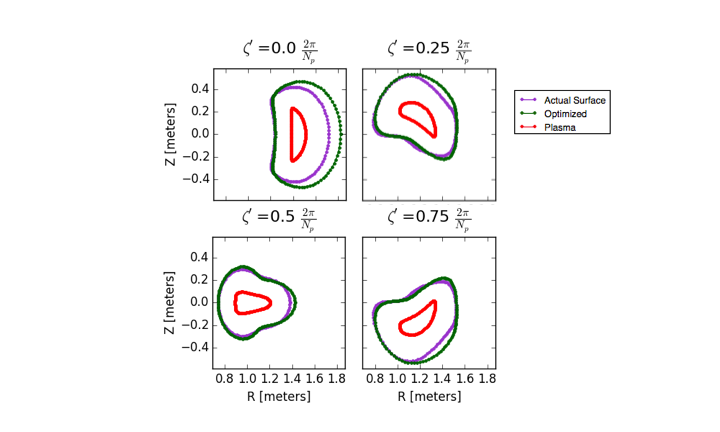
\includegraphics[width=1\textwidth]{hsx_opt_surf.png}
\caption{}
\end{subfigure}
\begin{subfigure}[b]{0.8\textwidth}
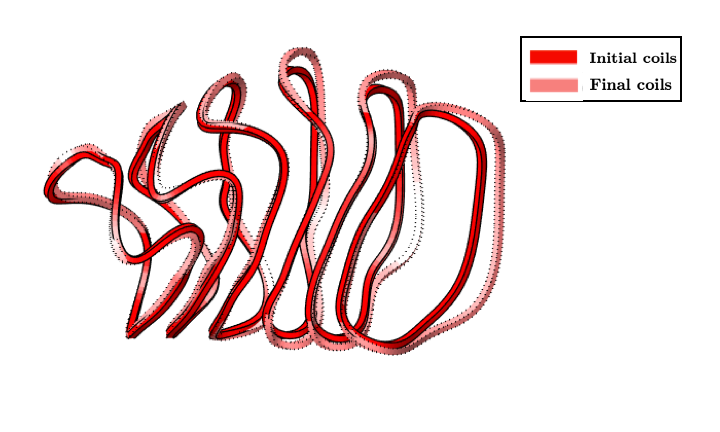
\includegraphics[width=0.8\textwidth]{hsx_opt_coils.png}
\caption{}
\end{subfigure}
\caption{(a) The actual HSX coil-winding surface and plasma surface are shown with the optimized winding surface. In comparison with the actual surface, the optimized surface has decreased $\chi^2_B$ by 4\% and increased $V_{\text{coil}}$ by 18\%. (b) The coils obtained from \texttt{REGCOIL} using the actual HSX winding surface (dark) and optimized surface (light).}
\label{fig_hsx}
\end{figure}

\begin{table}
\renewcommand{\arraystretch}{1.4}
\begin{tabular} {| c | c | c | c | c | c | c |}
\hline
& $\chi^2_B$ [T$^2$m$^2$] & $V_{\text{coil}}$[m$^3$] & $\norm{\bm{K}}_2$ [MA/m] & Mean $l$ [m] & Mean $\Delta \zeta'$ [rad.] & Mean $\kappa$ [m$^{-1}$] \\ \hline 
Initial & $1.53\times10^{-5}$ & 2.60 & 0.96 & 2.25 & 0.37 & 4.42 \\ \hline
Optimized & $1.47\times10^{-5}$ & 3.07 & 0.89 & 2.37 & 0.36 & 4.19 \\ \hline
Actual coilset & & & & 2.24 & 0.36 & 5.70 \\ \hline
\end{tabular}
\caption{Comparison of metrics of the winding surface and coilset for the HSX initial and optimized surfaces. The coil metrics for the actual HSX nonplanar coils are also shown. Regularization in \texttt{REGCOIL} is chosen such that the coil metrics computed on the initial surface roughly match those of the actual coilset.}
\label{table_hsx}
\end{table}

\FloatBarrier
\section{Winding surface sensitivity maps}
\label{sect_sensitivity}

With the adjoint method we have computed sensitivity derivatives of the objective function with respect to Fourier components of the winding surface, $\partial f/\partial \Omega$. While this representation of sensitivity derivatives is convenient for gradient-based optimization, visualization of the surface sensitivity in real space is obscured. Instead, we'd like to represent the sensitivity of $f$ with respect to normal displacements of surface area elements. 
\begin{gather}
d f(\Omega,\bm{V}) = \int_{\text{coil}} d^2 A \, S \left( \delta \bm{r}' \cdot \bm{n}' \right)
\label{shapederivative}
\end{gather}
The scalar $S$ will be called the surface sensitivity function. Intuitively, this form implies $f$ is insensitive to tangential displacements of the surface. The shape derivative is formally defined as follows \cite{Delfour2011}. Consider a velocity field, $\bm{V}$, which describes displacements of the surface, $\Omega$. The surface varies smoothly from $\Omega$ to $\Omega_t$, with the surface $\Omega_t$ given by the transformation $T_t$.
\begin{gather}
\Omega_t = \left \{ T_t(x_0) : x_0 \in \Omega \right \} \\
T_t(x) = x + t \bm{V}(x)
\end{gather}
The shape derivative, $df(\Omega,\bm{V})$, of a functional of the surface geometry, $f(\Omega)$, is defined in the following way. 
\begin{gather}
d f(\Omega, \bm{V}) = \lim_{t \rightarrow 0} \frac{ f(\Omega_t) - f(\Omega)}{t}
\end{gather}
Under some assumptions, the shape derivative can be represented in the form of equation \ref{shapederivative} as a consequence of the Hadamard-Zol\`{e}sio structure theorem \cite{Delfour2011}. This so-called Hadamard form for shape sensitivity derivatives is convenient for computation and has been applied for sensitivity maps of Navier-Stokes flow optimization for car aerodynamic design \cite{Othmer2008,Othmer2014}. It could have potential applications for stellarator design, allowing for visualization of regions on the winding surface which require tight engineering tolerances for a given figure of merit. 

As both $\chi^2_B$ and $\norm{\bm{K}}_2$ are defined in terms of surface integrals over the winding surface, it can be shown that the shape derivative of these functions takes the Hadamard form \cite{Novotny2013}. The surface sensitivity functions, $S_{\chi^2_B}$ and $S_{\norm{\bm{K}}_2}$, can be computed from the Fourier derivatives ($\partial \chi^2_B/\partial \Omega$ and $\partial \norm{\bm{K}}_2/\partial \Omega$) using a singular value decomposition method \cite{Landreman2018}. We have used this method to compute the surface sensitivity on the W7-X and HSX actual winding surfaces.  

For the W7-X surface (figure \ref{w7x_sensitivity}), the region of large $S_{\chi^2_B}$ is highly localized in the concave region on the inboard side. This corresponds to the bean cross-section at $\zeta' = 0$ (see figure \ref{fig_w7x}, subplot a). The surface sensitivity of $\norm{\bm{K}}_2$ is anti-correlated with that of $\chi^2_B$. This can be understood in light of equation \ref{regcoil_minimization}. As $\partial \chi^2_B/\partial \Phi_k$ increases $\partial \norm{\bm{K}}_2/\partial \Phi_k$ must decrease, since $\norm{\bm{K}}_2 = \sqrt{ \chi^2_K/A_{\text{coil}}}$. The Fourier sensitivity derivatives of these two quantities would also be related by the chain rule, equation \ref{sensitivity_der}. The inverse relationship between these two sensitivity functions demonstrates the tradeoff one must make between optimizing for physics properties (by decreasing $d_{\text{coil-plasma}}$ in the concave region) and optimizing for engineering properties (by increasing $d_{\text{coil-plasma}}$ for smoother coil shapes). Although the region of high sensitivity is not as well localized on the HSX surface (figure \ref{hsx_sensitivity}), we note that $S_{\chi^2_B}$ and $S_{\norm{\bm{K}}}$ are again anti-correlated. 

\FloatBarrier
\begin{figure}
\begin{subfigure}[b]{0.4\textwidth}
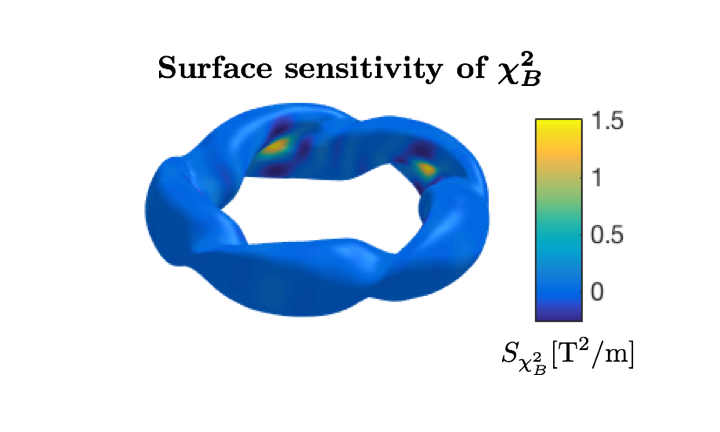
\includegraphics[width=1\textwidth]{chi2_B_S.png}
\end{subfigure}
\begin{subfigure}[b]{0.4\textwidth}
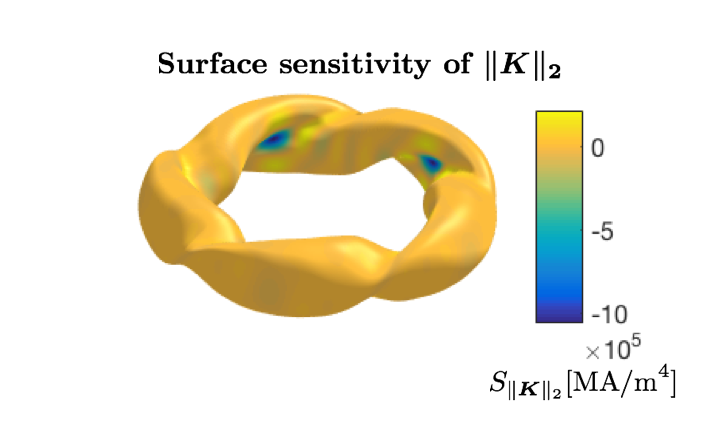
\includegraphics[width=1\textwidth]{rms_K_S.png}
\end{subfigure}
\caption{Surface sensitivity function, $S$, of $\chi^2_B$ and $\norm{\bm{K}}_2$ for the actual W7-X winding surface. }
\label{w7x_sensitivity}
\end{figure}
% x 0.65
% y 0.35
% width 0.03
% height 0.3
% chi2(B)
% theta_min = 1.9478
% zeta_min =1.2566
% theta_max = 3.1416
% zeta_max = 0
% rms(K)
% theta_min = 3.1416
% zeta_min = 0
% theta_max = 2.9531
% zeta_max = 6.0633

\begin{figure}
\begin{subfigure}[b]{0.4\textwidth}
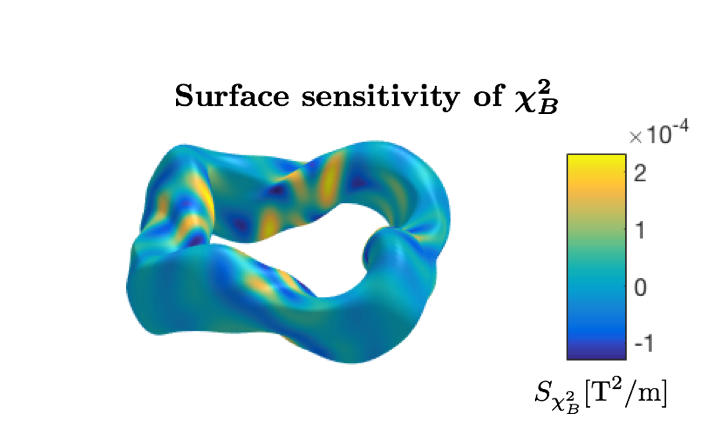
\includegraphics[width=1\textwidth]{chi2_B_S_HSX.png}
\end{subfigure}
\begin{subfigure}[b]{0.4\textwidth}
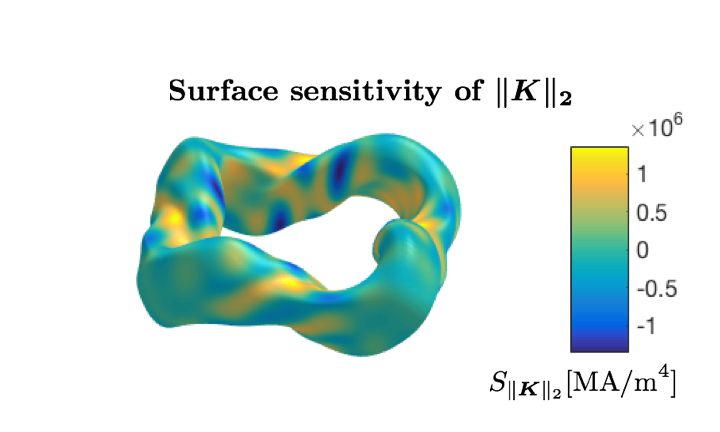
\includegraphics[width=1\textwidth]{rms_K_S_HSX.png}
\end{subfigure}
\caption{ Surface sensitivity function, $S$, of $\chi^2_B$ and $\norm{\bm{K}}_2$ for the actual HSX winding surface. }
\label{hsx_sensitivity}
\end{figure}
% x 0.7
% y 0.3
% width 0.04
% height 0.4
% RMS(K) 
% theta_min = 3.9898
% zeta_min = 5.8434
% theta_max = 5.1522
% zeta_max = 5.4350
% chi2_B
% theta_min = 3.4872
% zeta_min = 3.6757
% theta_max = 3.9584
% zeta_max = 2.7018

\FloatBarrier 

\section{Conclusions}
\label{sect_conclusions}

We have outlined a new method for optimization of the stellarator coil-winding surface using a continuous current potential approach. Rather than evolving filamentary coil shapes, we use \texttt{REGCOIL} to obtain the current density on a winding surface. We have shown that we can indirectly improve the coil curvature and toroidal extent by targeting the root-mean-squared current density in our objective function (figure \ref{rmsKcoilcompare}). Our approach offers several advantages over other nonlinear coil optimization tools.
\begin{enumerate}
\item The difficulty of the optimization is reduced by the application of the \texttt{REGCOIL} method, which takes the form of a linear least-squares system. The optimal coil shapes on a winding surface can thus be efficiently and robustly computed. 
\item By fixing the maximum current density in order to obtain the regularization in \texttt{REGCOIL}, we eliminate the need to implement an additional equality constraint or arbitrary weight in the objective function. 
\item By using \texttt{REGCOIL} to compute coil shapes on a given surface, we are able to apply the adjoint method for computing sensitivity derivatives (section \ref{sect_adjoint}). This allows us to minimize the number of function evaluations required during the nonlinear optimization. 
\end{enumerate} 
We have demonstrated this method by optimizing the actual W7-X and HSX winding surfaces (figures \ref{fig_w7x} and \ref{fig_hsx}). We find that we are able to simultaneously decrease the integrated-squared error in reproducing the plasma surface, increase the volume contained within the winding surface, maintain the minimum coil-plasma distance, and improve the coil metrics over those of the initial winding surfaces (tables \ref{table_w7x} and \ref{table_hsx}). 

There are several limitations of this approach that should be noted. First, we have applied a local nonlinear optimization algorithm. This is a reasonable choice if the initial condition is close to a global optimum. We note that the NLOPT package features several global gradient-based routines which could be applied if necessary. Second, while the current potential approach is robust, we are limited in the metrics we can include in our objective function. It is difficult to, for example, target the coil curvature separately from the length.

While the sensitivity derivatives computed are with respect to Fourier coefficients of the winding surface, we demonstrate a technique for their visualization in real space. This surface sensitivity function describes how an objective function changes with respect to normal displacements on the winding surface. We apply this technique to the derivatives of the integrated-squared $B_n$ on the plasma surface and the root-mean-squared current density on the winding surface, finding them to be anti-correlated (figures \ref{w7x_sensitivity} and \ref{hsx_sensitivity}). This visualization technique could have potential applications for quantification of engineering tolerances in stellarator design. 

We have illustrated the application of adjoint methods to gradient-based optimization of the stellarator winding surface and for visualization of surface sensitivities. As stellarators feature complex geometry with many free parameters describing a given configuration, this field could benefit from further incorporation of these methods in other aspects of the design process, such as computation of neoclassical transport and magnetic equilibria. 

\appendix

\section{Adjoint sensitivity derivative at fixed $K_{\text{max}}$}
\label{lambda_search}
We enforce $K_{\text{max}}$ in the \texttt{REGCOIL} solve in order to obtain the regularization parameter, $\lambda$, by requiring that the following constraint be satisfied within some tolerance. 
\begin{gather}
G(\Omega, \bm{\Phi}(\Omega)) = K_{\text{max}}(\lambda) - K^{\text{target}}_{\text{max}}  = 0 
\label{K_constraint}
\end{gather}
Here $K^{\text{target}}_{\text{max}}$ is the target maximum current density. We need to compute sensitivity derivatives similar to equation \ref{adjointsensitivity} subject to this constraint. A log-sum-exponent function is used to approximate the maximum function, similar to that used to approximate $d_{\text{coil-plasma}}$ (equation \ref{lse_d}).
\begin{gather}
K_{\text{max}} \approx K_{\text{max},\, \text{lse}} =  \frac{1}{p} \log \left( \frac{\int_{\text{coil}} d^2 A \,  \exp\left(p K\right)}{ \int_{\text{coil}} d^2 A } \right)
\end{gather}
The derivative of $\bm{\Phi}$ with respect to $\Omega_j$ subject to equation \ref{K_constraint} in addition to the forward equation (equation \ref{forward}), is given by the following expression. 
\begin{multline}
\partder{\bm{\Phi}}{\Omega_j} \bigg \rvert_{A \bm{\Phi} = \bm{b}, \, G = 0} = - A^{-1} \left( \partder{A}{\Omega_j} \bm{\Phi} - \partder{\bm{b}}{\Omega_j} \right)\\ - \frac{A^{-1} \left( A^K \bm{\Phi} - \bm{b}^K \right) }{ \partder{G}{\bm{\Phi}} \cdot \left[ A^{-1} \left( A^K \bm{\Phi} - \bm{b}^K \right) \right] } \left( \partder{G}{\Omega_j} - \partder{G}{\bm{\Phi}} \cdot \left[ A^{-1} \left( \partder{A}{\Omega_j} \bm{\Phi} - \partder{\bm{b}}{\Omega_j} \right) \right] \right) 
\end{multline}
Here $A^K = \partder{A}{\lambda}$ and $b^K = \partder{b}{\lambda}$. We use the adjoint method to avoid inverting the operator $A$ for each $\Omega_j$.
\begin{multline}
\partder{\bm{\Phi}}{\Omega_j} \bigg \rvert_{A \bm{\Phi} = \bm{b}, \, G = 0} = - A^{-1} \left( \partder{A}{\Omega_j} \bm{\Phi} - \partder{\bm{b}}{\Omega_j} \right)\\ - \frac{A^{-1} \left( A^K \bm{\Phi} - \bm{b}^K \right) }{ \left[ \left( A^T \right)^{-1} \partder{G}{\bm{\Phi}} \right] \cdot \left( A^K \bm{\Phi} - \bm{b}^K \right) } \left( \partder{G}{\Omega_j} - \left[ \left( A^T \right)^{-1} \partder{G}{\bm{\Phi}} \right]  \cdot \left( \partder{A}{\Omega_j} \bm{\Phi} - \partder{\bm{b}}{\Omega_j} \right) \right) 
\label{withadjoint}
\end{multline}
So, we need to solve an additional adjoint equation for $\tilde{\bm{q}}$.
\begin{gather}
A^T \tilde{\bm{q}} = \partder{G}{\bm{\Phi}}
\label{adjoint_2}
\end{gather}
Equation \ref{withadjoint} is used to compute the sensitivity derivatives of $\chi^2_B$ with respect to $\Omega$.
\begin{gather}
\partder{\chi^2_B}{\Omega_j} \bigg \rvert_{A \bm{\Phi} = \bm{b}, \, G = 0} = \partder{\chi^2_B}{\Omega_j} \bigg \rvert_{\bm{\Phi}, \lambda} - \partder{\chi^2_B}{\bm{\Phi}} \cdot \partder{\bm{\Phi}}{\Omega_j} \bigg \rvert_{A \bm{\Phi} = \bm{b}, \, K_{\text{max}} = K_{\text{max}}^{\text{target}}}
\end{gather}
This can be written in terms of both adjoint variables, $\bm{q}$ and $\tilde{\bm{q}}$. 
\begin{multline}
\partder{\chi^2_B}{\Omega_j} \bigg \rvert_{A \bm{\Phi} = \bm{b}, \, G = 0} = \partder{\chi^2_B}{\Omega_j} \bigg \rvert_{\bm{\Phi}, \lambda} - \bm{q} \cdot \left( \partder{A}{\Omega_j} \bm{\Phi} - \partder{\bm{b}}{\Omega_j} \right) - \frac{ \bm{q} \cdot \left(A^K \bm{\Phi} - \bm{b}^K \right)}{  \tilde{\bm{q}} \cdot \left( A^K \bm{\Phi} - \bm{b}^K \right) } \left( \partder{G}{\Omega_j} - \tilde{\bm{q}} \cdot \left( \partder{A}{\Omega_j} \bm{\Phi} - \partder{\bm{b}}{\Omega_j} \right) \right)
\end{multline}
The same method is used to compute sensitivity derivatives of $\norm{\bm{K}}_2$. So, to obtain the sensitivity derivatives at fixed $K_{\text{max}}$, we compute a solution to the two adjoint equations, \ref{adjoint} and \ref{adjoint_2}, in addition to the forward equation, \ref{forward}.

\section*{Acknowledgements}
The authors would like to thank I. Abel for helpful input and discussions. This work was supported by the US Department of Energy through grants DE-FG02-93ER-54197 and DE-FC02-08ER-54964. The computations presented in this paper have used resources at the National Energy Research Scientific Computing Center (NERSC). 

\raggedright
\bibliographystyle{apsrev4-1}
\bibliography{AdjointRegcoil.bib}

\end{document}